\documentclass[12pt, a4paper, twoside]{article}

\usepackage[utf8]{inputenc}
\usepackage[T1]{fontenc}
\usepackage[english]{babel}

%\usepackage{layout}
%\usepackage{geometry}
%\usepackage{setspace}
\usepackage{soul}
\usepackage{ulem}
%\usepackage{eurosym}

%\usepackage{bookman}
%\usepackage{charter}
%\usepackage{newcent}
%\usepackage{lmodern}
%\usepackage{mathpazo}
%\usepackage{mathptmx}

%\usepackage{url}
%\usepackage{verbatim}
%\usepackage{moreverb}
\usepackage{listings}
%\usepackage{fancyhdr}
%\usepackage{wrapfig}
%\usepackage{color}
%\usepackage{colortbl}

\usepackage{amsmath}
\usepackage{amssymb}
\usepackage{mathrsfs}
%\usepackage{asmthm}

%\usepackage{makeidx}

\usepackage{graphicx}
\usepackage{caption}
\usepackage{blindtext}

\title{\huge{\textbf{Eye-Assisted Text Editing }\\ Future User Interfaces}}
\author{Gwenael \textsc{Gendre}, Lionel \textsc{Ieri}, Romain \textsc{Maillard} \\
	Teacher: Prof. Dr. Denis \textsc{Lalanne}}
\date{Summer 2018}
 
\begin{document}
 
\begin{titlepage}
\maketitle
\end{titlepage}
\tableofcontents
\newpage

\section{Introduction}
During the \textit{Future User Interfaces} course at the University of Fribourg, we had to develop and implement a multimodal interface, using eye tracking, keyboard and/or mouse. Thanks to a collaboration with \textit{Logitech}, each group could use the \textit{Tobii Eye Tracker 4C}. 

\section{Outline}

\subsection{Motivation}
The idea we had was to facilitate the text editing of documents, mostly for users that do not use the many shortcuts implemented in almost all of the modern text editing softwares. These shortcuts are very powerful in some cases (see e.g. \textit{Vim}) but these solutions have extremely long lists of shortcuts and macro that are not user friendly.\\
A user wanting to edit text will therefore have to open menus and select the right options with the mouse, either to change the font or its size, to navigate the spellchecker or to save and send the file. The user has to put his hands away from the keyboard and loses time and comfort for each of these movements. \\
We wanted to build an interface that could allow such users to have an easier way of editing their documents. 

\subsection{Concept}
Our project has a custom text editor built in, in which the user can choose to activate -- or deactivate -- the eye assisted text editing. Without eye-tracking, the user has a text editor with the usual commands: one can type text, change the font and its size, save the file or open another one, and spellcheck the typed text. By checking the corresponding box, the user activates the eye assistance. The mouse controls still remain available, but more possibilities appear: as stated on the left on the window, there are two keys that can be pressed: \textit{AltGr} activates scrolling: look at the top or the bottom of the text field and press \textit{AltGr}, the field will scroll up or down. When the user presses the \textit{Right Shift} key, two things can happen. Either he was not looking at the text field, and a menu with big icons opens, easier to focus with your gaze. There are five options in this menu: open a file, saving the current text field as a file, open the style editor, open the spell checker or exit the application. The style editor allows to change the font and the size of the text, while the spellchecker displays the suggestions for the word. Or the user was in fact looking at the text field, and the spellcheck directly opens. Note that the options have to be selected by pressing the \textit{Right Shift} key again. 

\subsection{CASE/CARE}
According to the \textit{CASE} model, our application is synergistic: we use the two modalities (keyboard and eye) in parallel, and both accomplish the same action. (See Figure \ref{case-model})
\begin{figure}\centering
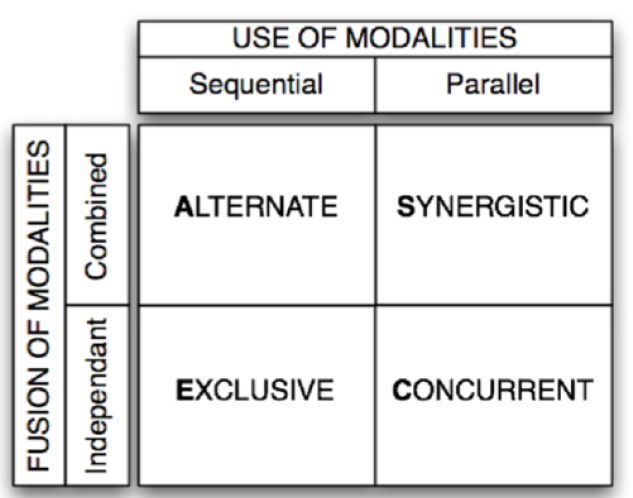
\includegraphics[scale=0.9]{casecare}
\caption{The CASE model}
\label{case-model}
\end{figure}
\newline
The \textit{CASE} model classified the machine-side of the fusion, now the \textit{CARE} model is about the human-side of fusion and classifies the usability properties: in our application, the two modalities are complementary. We need to use both of them at the same time to use correctly the application. 

\subsection{Fusion and fission}
We use \textit{decision-level fusion}: we merge lately the two modalities (the gaze position and the key pressing) because they are weakly coupled. On the fission side, it is a bit hard to have two different outputs for the user: we kept the feedback visual by highlighting the gazed-at element and by letting the menus appear directly upon a key press.  

\section{Architecture}

\subsection{Hardware}
The main hardware used for this project is a \textit{Tobii EyeTracker 4C}, a USB eye tracker using an infrared camera to track the gaze position and translate it to the screen. This system is relatively low cost and works well enough for many usages, as unlike more expensive systems, the point of the \textit{4C} isn't to properly track every single movement but more to determine the different areas gazed upon. 
And for our project we will use it in coordination with a standard keyboard.

\subsection{Software}
To be able to access the \textit{Tobii} gaze data, we used the \textit{Tobii Core Standard Development Kit}\footnote{https://developer.tobii.com/tobii-core-sdk/} and its provided \textit{API}s. We then decided not to implement a plugin for an already existing text editor but rather to create our own one. The \textit{Windows Presentation Foundation}\footnote{https://msdn.microsoft.com/fr-fr/library/aa970268(v=vs.100).aspx} was all we needed: windows creation with built-in text fields and style modification. The \textit{WPF} uses the \textit{XAML} language. 

\subsection{Implementation}
The integration of the \textit{Tobii} in our application is quiet easy. There is a good synergy between \textit{WPF} and the \textit{Tobii SDK}. We can add some parameter to the element of a window to add the capacity to use the eye tracker.

\begin{lstlisting}
<Button x:Name="validation"
wpf:Behaviors.IsActivatable="True"
wpf:Behaviors.IsTentativeFocusEnabled="True"
wpf:Behaviors.Activated="activation_function">
\end{lstlisting}

The above example of code allows a button to be activated by the eye tracker. When it is activated, it calls the function \textit{activation\_function}.

\subsubsection{In the app}
We use the eye tracker in our application as follows:
\begin{itemize}
\item Scroll the text
\item Quick menu for the main function of the application
\item Select the style of the text
\item Correct spelling mistakes
\end{itemize}

\section{Data analysis}

\subsection{Hypothesis}
We hope to see a significant amelioration in the text editing quality by using our application. Therefore we can formulate our null hypothesis as follows: 
\[H_0: \text{There is no increase in speed by editing text with the eye tracker.}\] 
along with the alternative hypothesis: 
\[H_1: \text{Editing text with eye tracker support is faster than without it.}\]

\subsection{Protocol}

\subsubsection{Discovery}
We let the user take a couple of tries with the system to avoid stressing them during the actual experiment and to let them learn how to use it. 

\subsubsection{Test}
The user was first asked to copy a given short text with a precise formatting, e.g. different fonts and font sizes. Then we asked him to correct some spelling mistakes on another text, which may require scrolling. This was done either with the eye-tracking interface or with the classical one. \\
We then swapped to the other modality choice and asked the user to repeat the task on the same text. \\
The time for both parts was measured. 

\subsubsection{Evaluation}
The user then filled a form to gather their feedback and impression. This form touched upon personal preferences, potential (does the user feel like he could become more proficient with more experience), issues and ideas. 

\subsection{Experiment}

\subsection{Analysis and results}


\section{Conclusion}
 
\end{document}

